\chapter{Résultats}
\label{chap:Résultats}

Dans l'ensemble, les résultats sont plutôt décevants.
En effet, les modèles n'ont pas réussi à prédire les résultats avec de meilleure performance que le modèle de base.
Cependant, il est possible de tirer quelques enseignements de ces résultats comme le fait que \acrshort{svm} n'est pas fait pour les larges set de données ou que la normalisation n'est pas forcément un facteur important.


% -----------------------------------------------------------------------------
\section{Récoltes des données}

Tous les noms de molécules ne sont pas traductible en \acrshort{smiles}.
De plus, la librairie mordred n'arrive pas à calculer les descripteurs pour toutes les molécules.
C'est pourquoi, nous avons quelques pertes sur les nouvelles données.
Le nombre de liquides ioniques était de 765 et il est passé à 739 ce qui nous fait une perte de 3,4\%.
Si on regarde l'implication sur les datasets, nous avons le training set qui passe de 600 à 583 et le test set qui passe de 168 à 159.
Ceci fait respectivement une baisse de 2,8\% et 5,4\%.
Les données ont déjà été complétée à la main par Chemtech.

% -----------------------------------------------------------------------------
\newpage
\section{Choix des modèles}
En prenant les nouvelles données non normalisées et en utilisant les paramètres par défaut des modèles, nous pouvons nous faire une idée de la performance de chacun et des résultats qu'ils donnent.

\begin{figure}[ht]
    \centering
    \subfloat[\centering \acrshort{nusvr} avec les paramètres de Mme Yerly]{{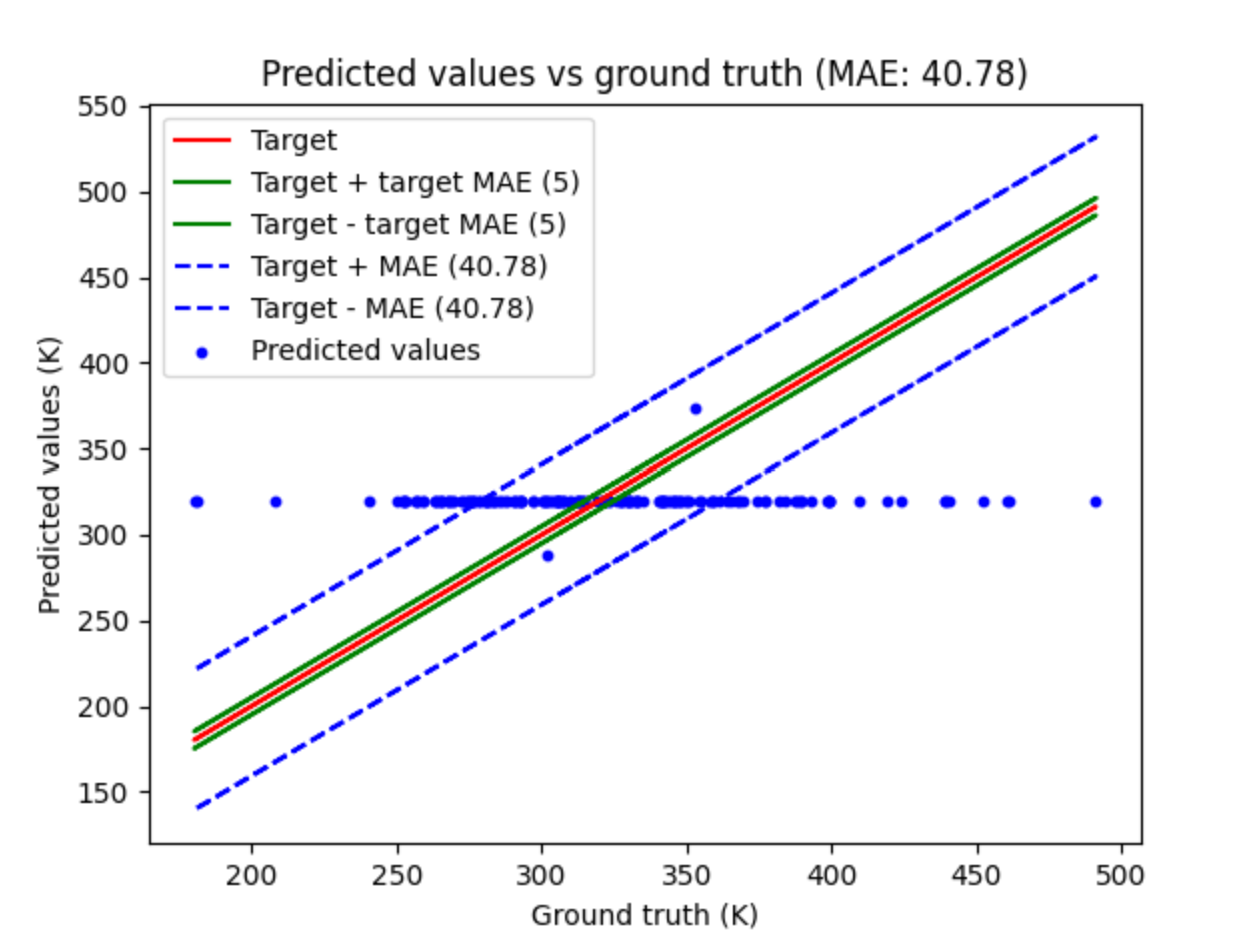
\includegraphics[width=60mm]{img/result_nusvr_noNorm.png}}}
    \qquad
    \subfloat[\centering \acrshort{svm}]{{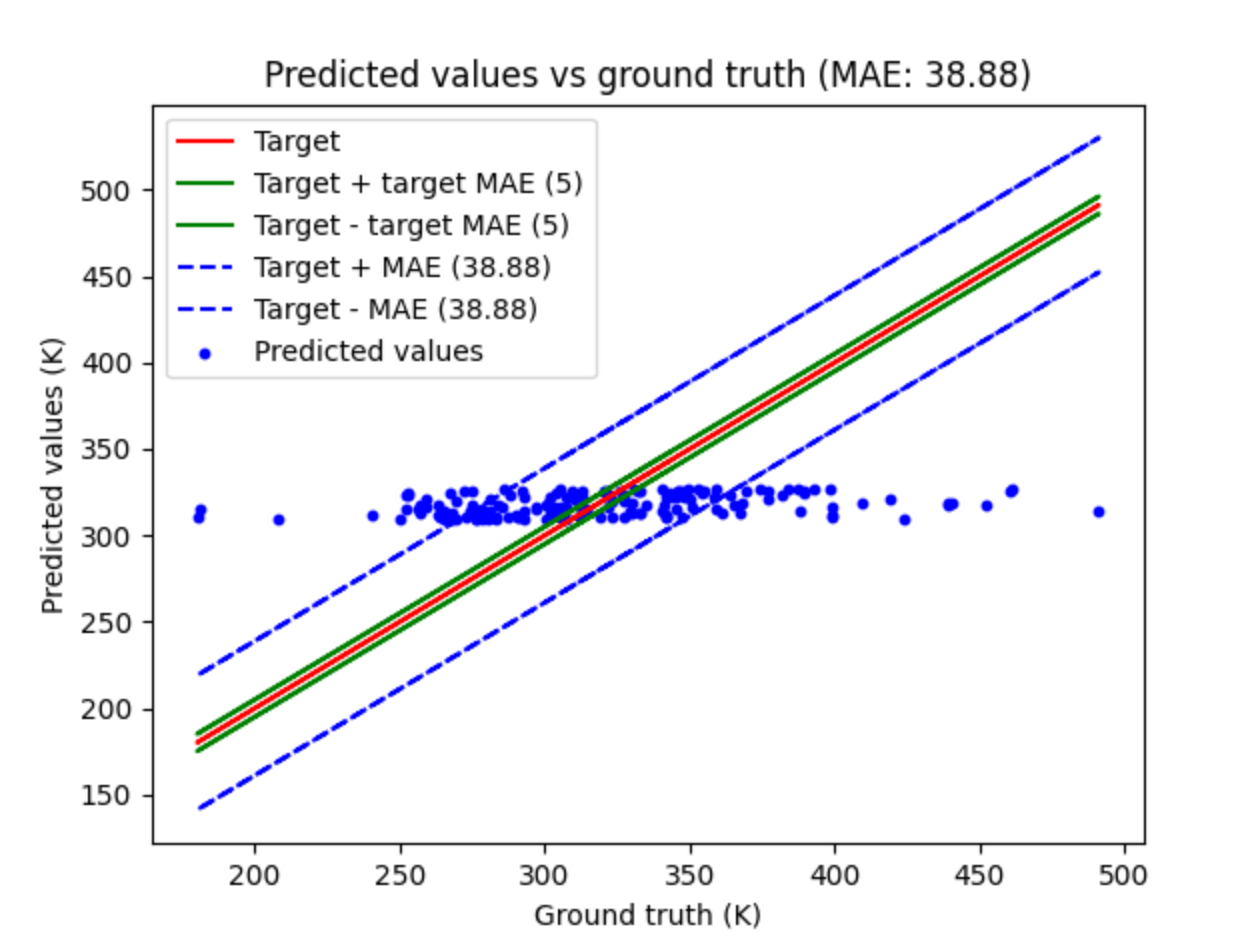
\includegraphics[width=60mm]{img/result_svr_noNorm.png}}}
    \qquad
    \subfloat[\centering Random forest]{{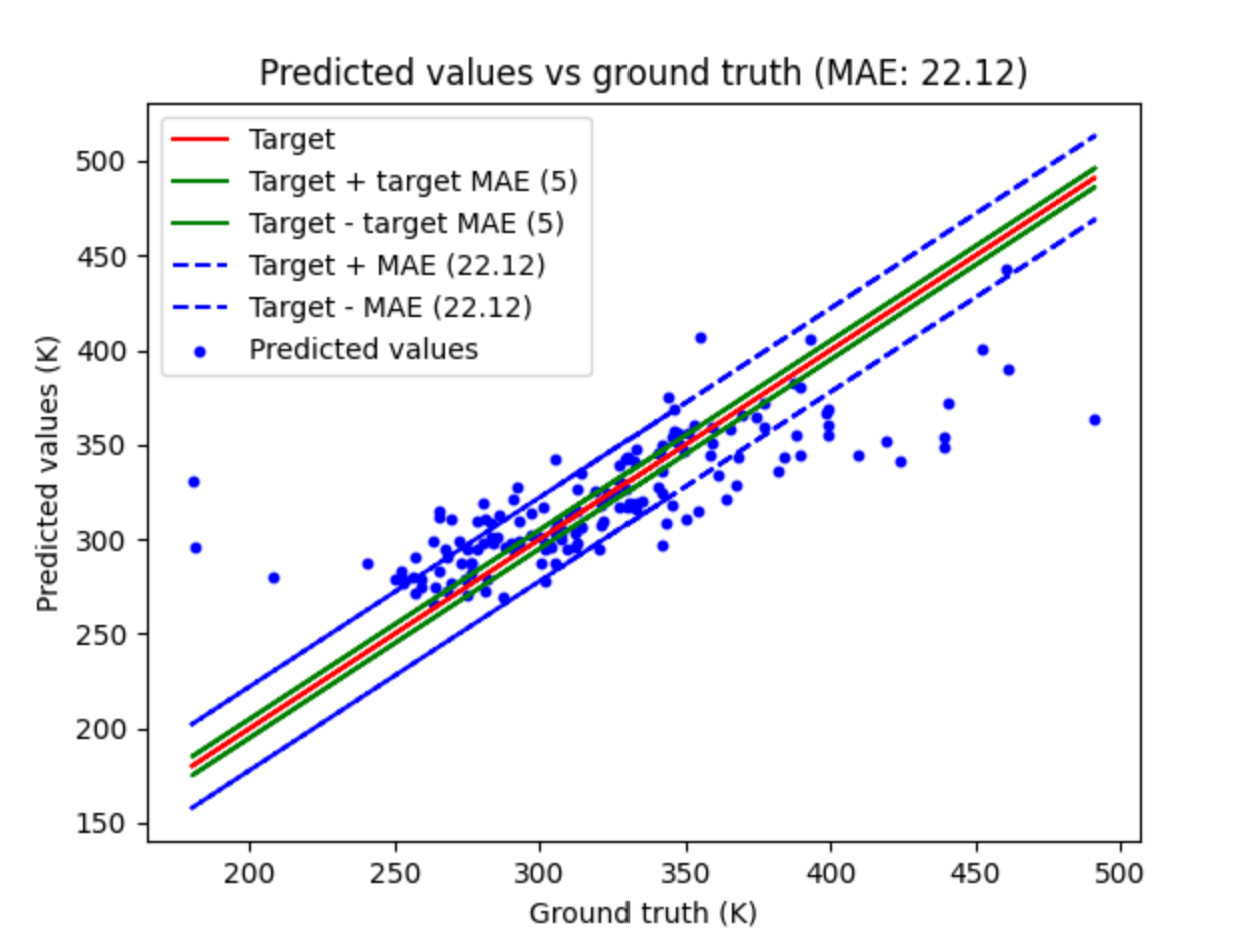
\includegraphics[width=60mm]{img/result_rf_noNorm.png}}}
    \qquad
    \subfloat[\centering Gradient boosting]{{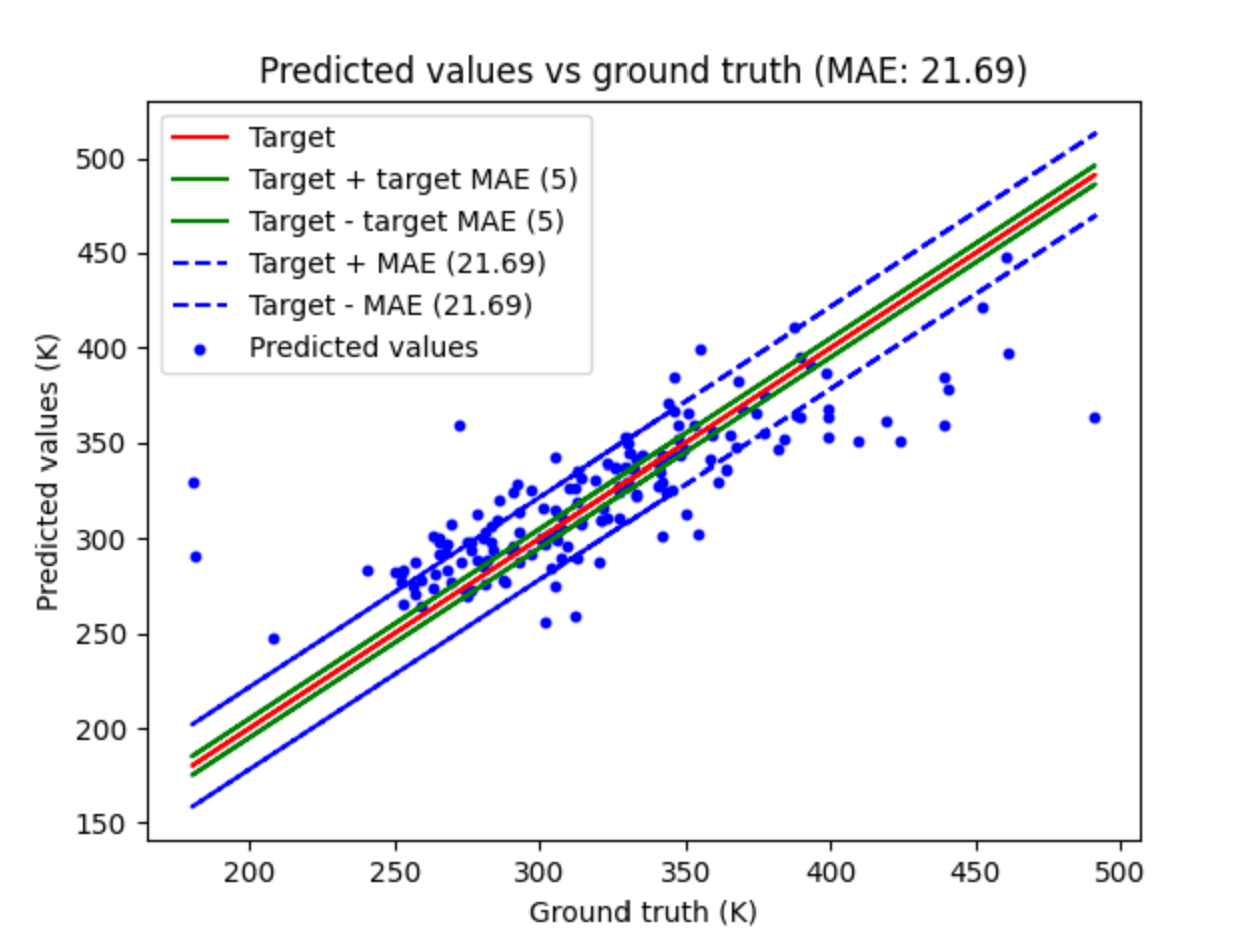
\includegraphics[width=60mm]{img/result_gb_noNorm.png}}}
    \captionof{figure}{Résultats des modèles avec les paramètre par défaut sans normalisation ni preprocessing}
\end{figure}

Ce qui ressort c'est que \acrshort{svm} n'est pas performant avec un large set de données.
Ce qui est flagrant c'est la difficulté qu'ont les modèles à prédire les données et ils font un compromis pour mettre toutes les données dans la moyenne.


\newpage
\subsection{Normalisation}
Les résultats étant très mauvais sur les \acrshort{svm}, ils seront écartés de la suite des expériences.
La normalisation est un facteur important dans la modèle de régression.

\begin{figure}[ht]
    \centering
    \subfloat[\centering Random forest normalisé avec \acrshort{minimax}]{{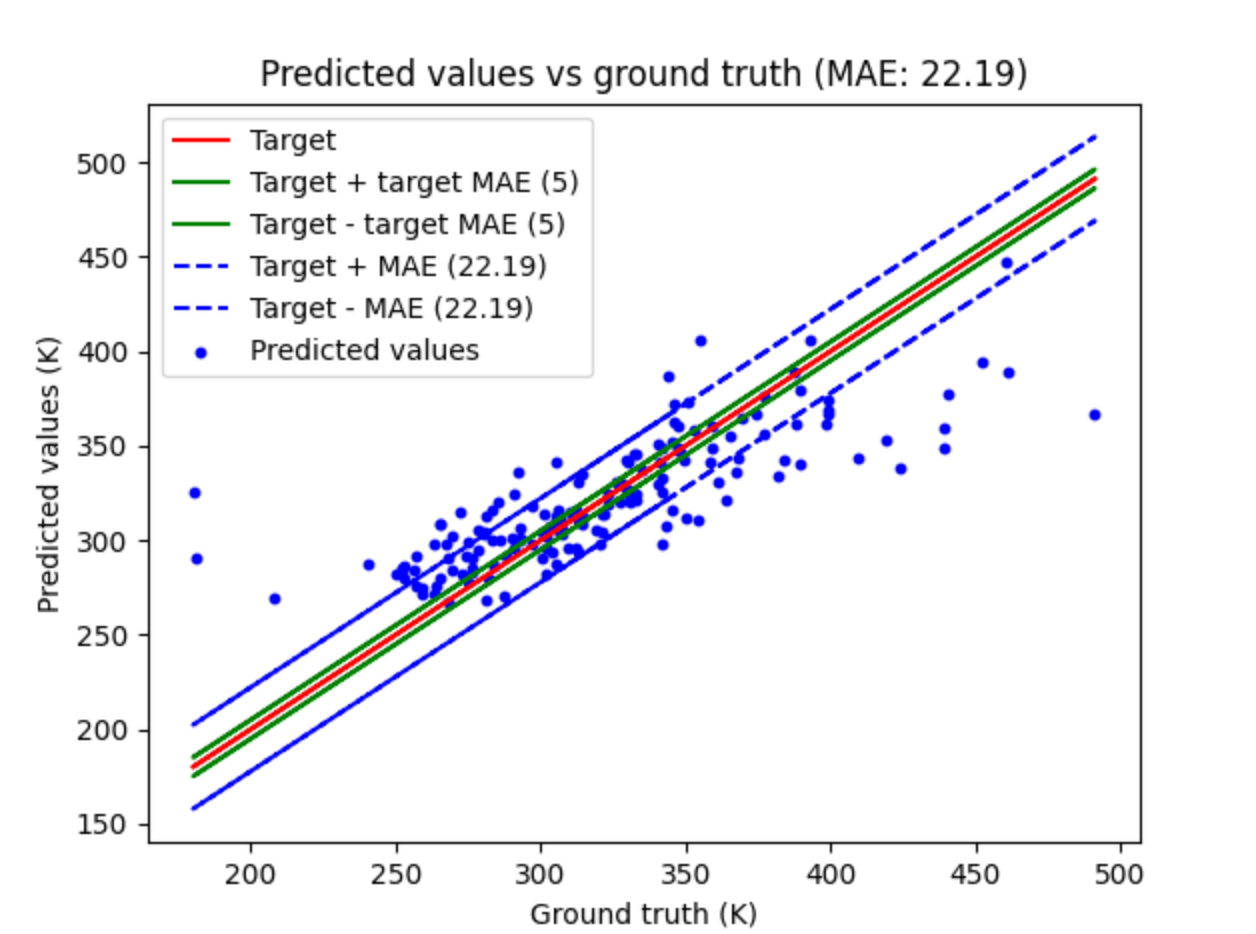
\includegraphics[width=60mm]{img/result_rf_minmax.png}}}
    \qquad
    \subfloat[\centering Gradient boosting normalisé avec \acrshort{minimax}]{{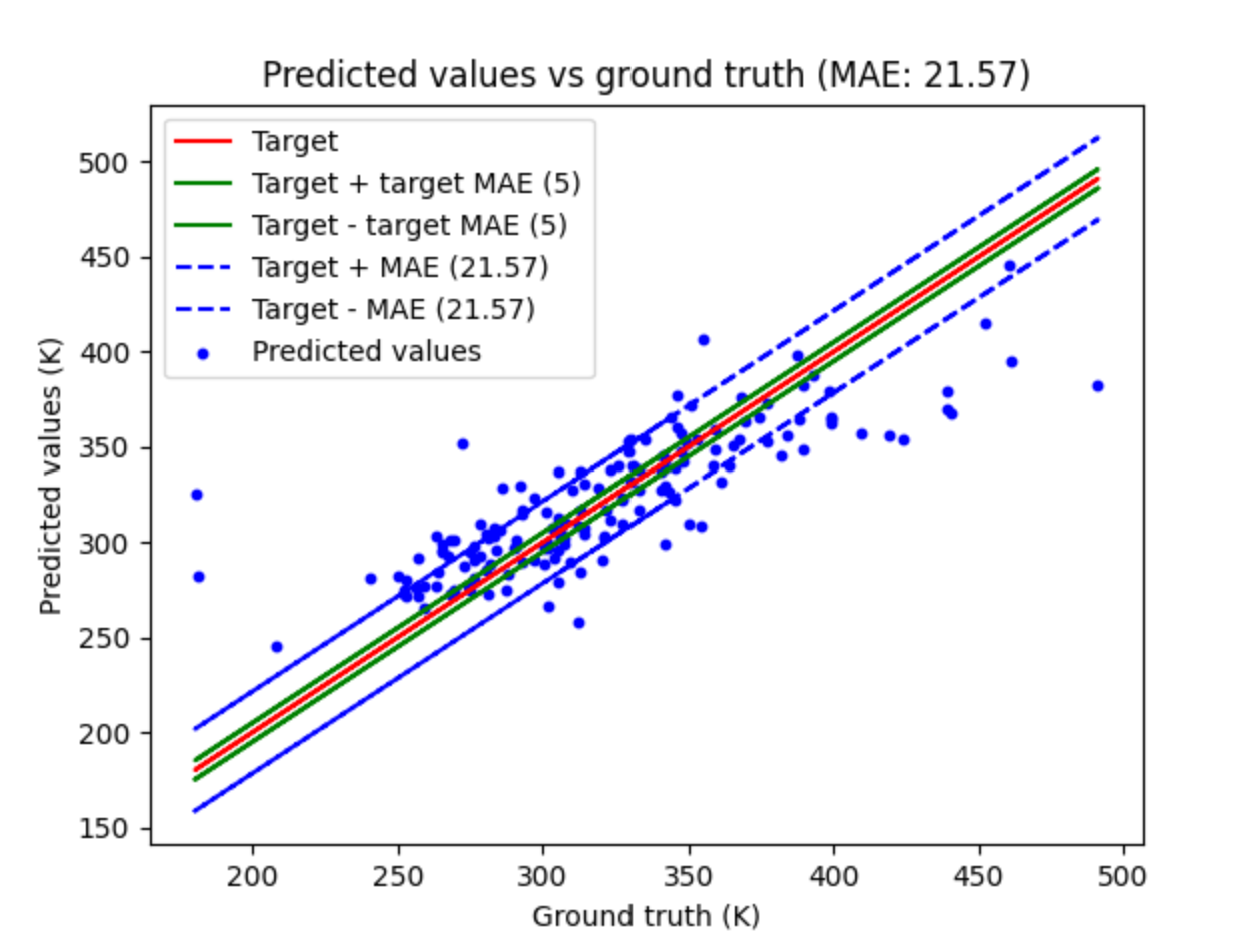
\includegraphics[width=60mm]{img/result_gb_minmax.png}}}
    \qquad
    \subfloat[\centering Random forest standardizé]{{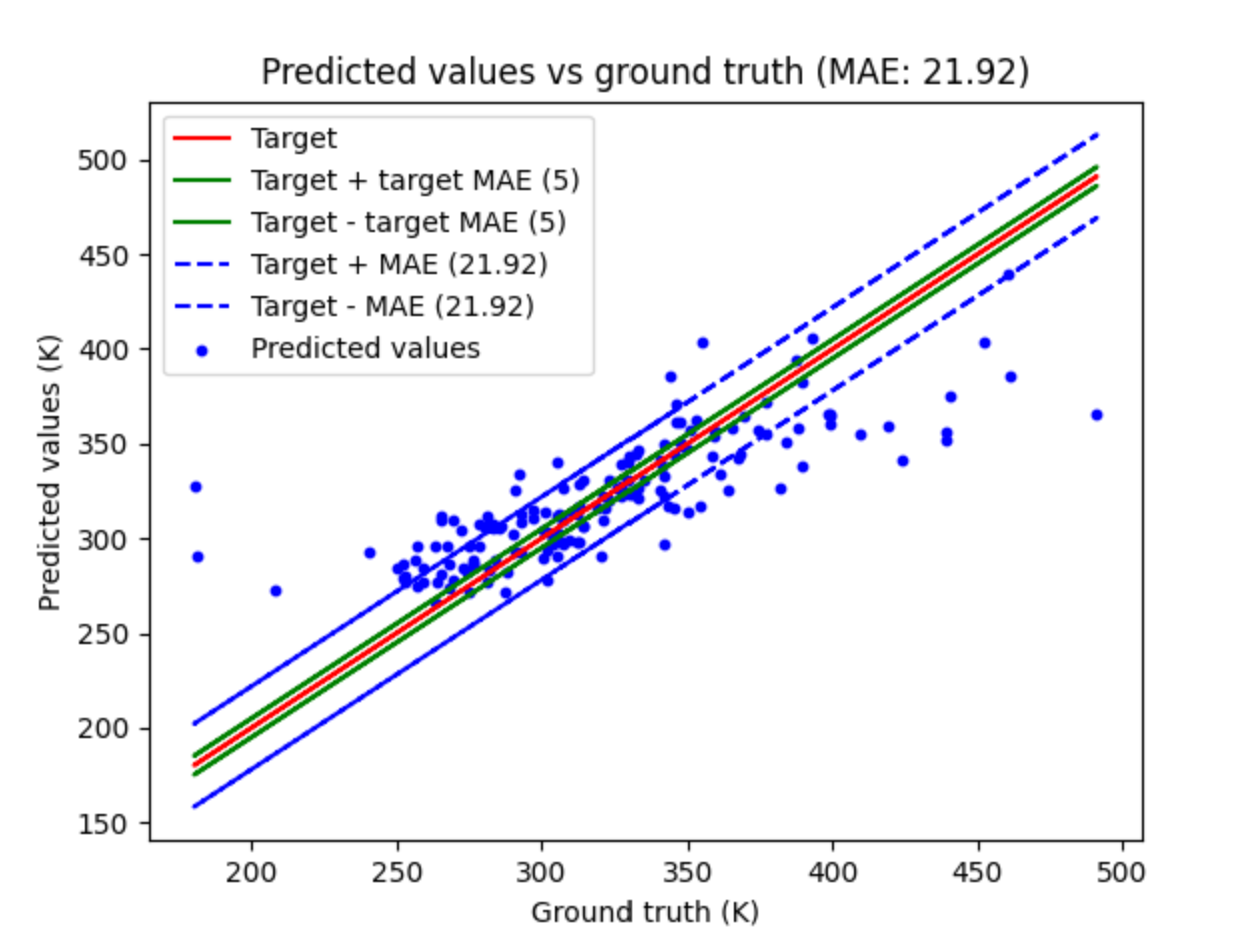
\includegraphics[width=60mm]{img/result_rf_standard.png}}}
    \qquad
    \subfloat[\centering Gradient boosting standardizé]{{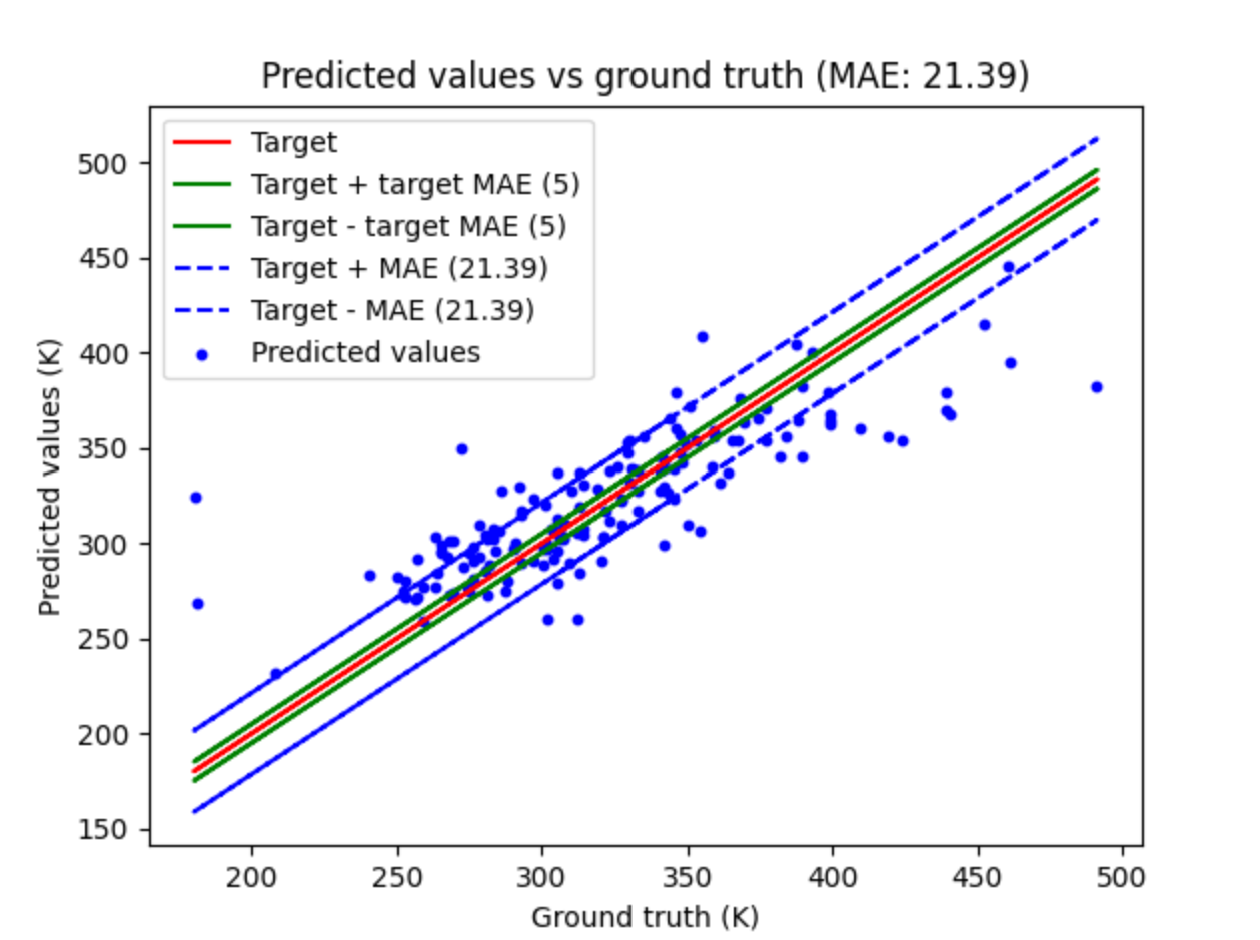
\includegraphics[width=60mm]{img/result_gb_standard.png}}} 
    \captionof{figure}{Résultats des modèles avec les paramètre par défaut et différente normalisation}
\end{figure}

Les résultats ne s'améliorent pas significatievement avec la normalisation.

\subsection{Autres axes}
D'autre axes d'améliorations ont été explorer comme le \acrfull{pca} mais les résultats étaient similaires.
Une hypothèse intéressante était de fusionner les nouvelles données avec les données de Mme Yerly et de voir si les modèles obtenaient les mêmes résultats que lors de la reproduction.
Si cette s'étaiet vérifié, cela aurait indiqué que les nouvelles données n'apportaient rien de plus.
Malheureusement, les résultats n'étaient pas mieux mais les features sélectionnées faisaient partie des deux jeux de données.


